\chapter{Image segmentation}

\section{Problem statement}

\begin{enumerate}[(a)]
    \item Develop a program to implement the Roberts, Prewitt,
Sobel, the Marr-Hildreth and the Canny edge detectors. Use the
image ‘building.tif’ to test your detectors. (For technique details
of Marr-Hildreth and Canny, please refer to pp.736-747 (3rd
edition, Gonzalez DIP) or MH-Canny.pdf at the same address of
the slides.)

    \item Develop a program to implement the Otsu’s method of
thresholding segementation, and compare the results with the
global thresholding method using test image ‘polymersomes.tif.
(For technique details, please refer to pp.763-770 (3rd edition,
Gonzalez DIP), or Otsu.pdf at the same ftp address of slides.)

\end{enumerate}


\section{Python implementation}
\bigskip
Three programs: \\
\begin{itemize}
    \item Marr-Hildreth edge detector: \textbf{marr.py}

    Usage:~\textbf{marr.py [-h] [-s SIGMA] image\_path} \\
    Use \textbf{python marr.py -h} to see the help.

    \bigskip

    \item Canny edge detector: \textbf{canny.py}

    Usage:~\textbf{canny.py [-h] (--roberts | --sobel | --prewitt) [-s SIGMA]} \\
           \textbf{[--th TH] [--tl TL] image\_path} \\
    Use \textbf{python canny.py -h} to see the help.

    \bigskip

    \item Otsu's method of thresholding segmentation: \textbf{otsu.py}

    Usage:~\textbf{otsu.py [-h] [-o] [-g] image\_path} \\
    Use \textbf{python otsu.py -h} to see the help.

\end{itemize}


\pagebreak

\section{Marr-Hildreth edge detector}

    \textbf{python marr.py -s 4 building.tif}

    \begin{figure}[!htb]\centering
        \begin{minipage}{0.8\textwidth}
            \frame{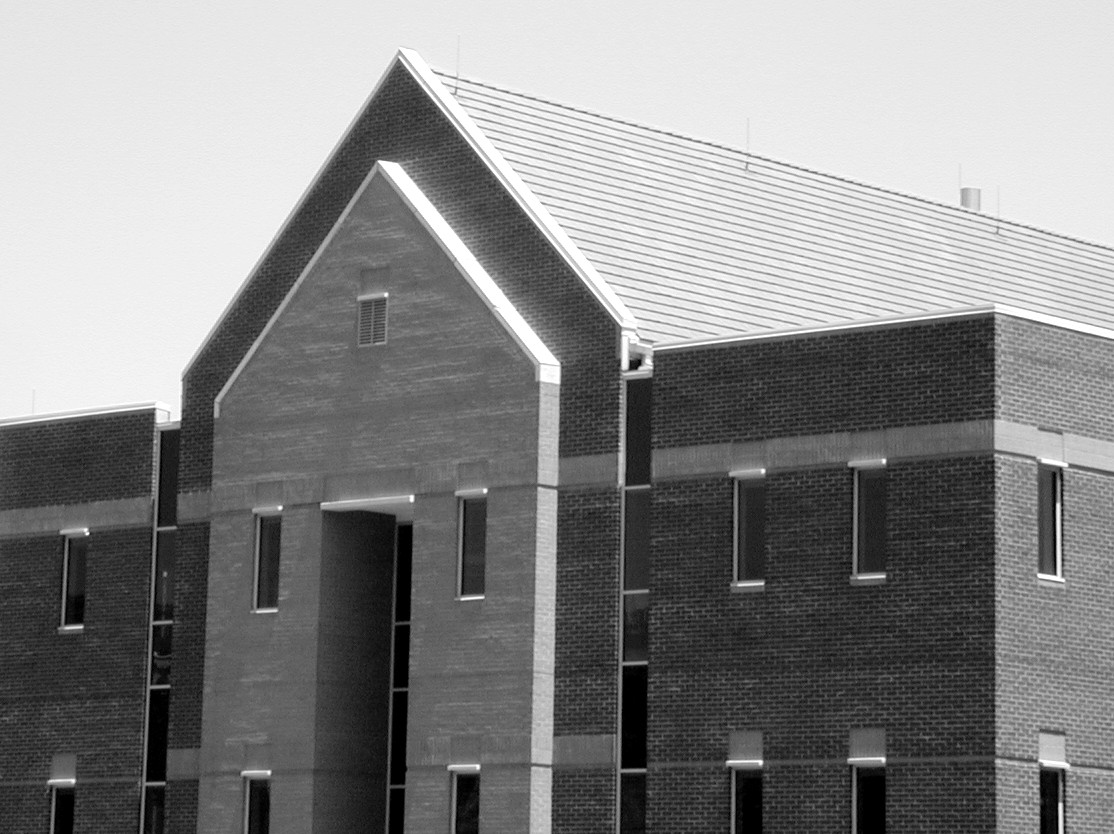
\includegraphics[width=\linewidth]{./images/9/building.jpg}}
            \caption{\small{Original image}}\label{diagram:building}
        \end{minipage}
    \end{figure}

    \begin{figure}[!htb]\centering
        \begin{minipage}{0.8\textwidth}
            \frame{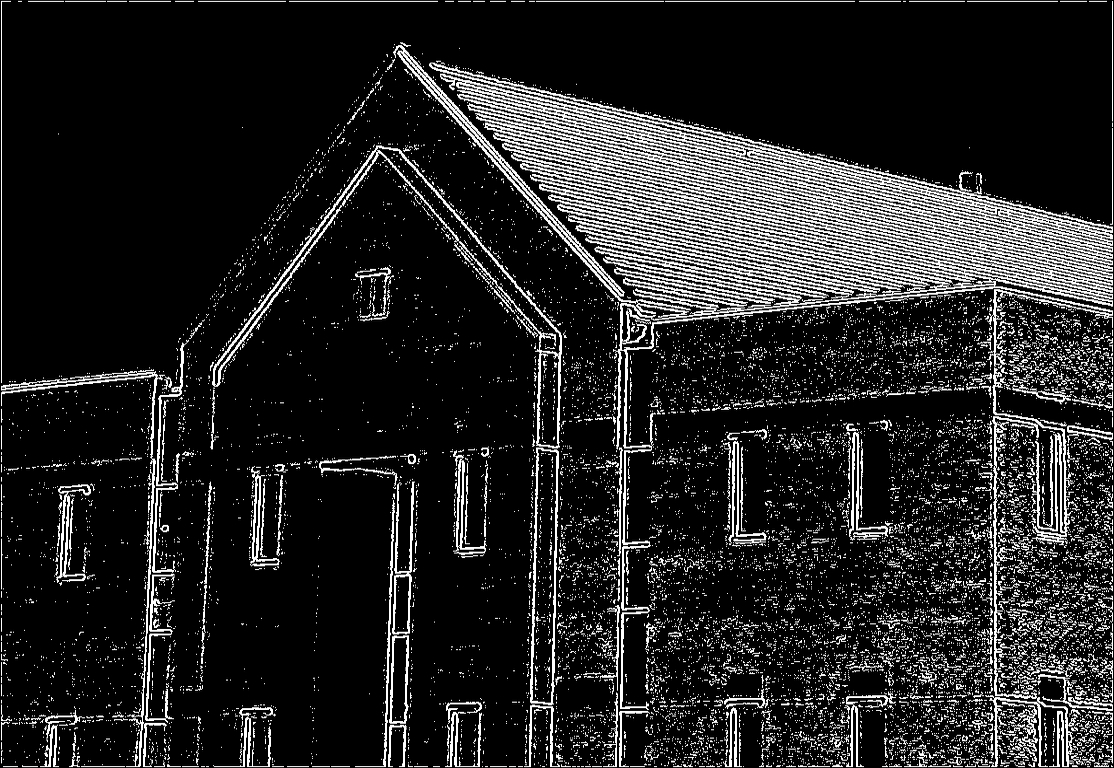
\includegraphics[width=\linewidth]{./images/9/marr.jpg}}
            \caption{\small{Marr-Hildreth}}\label{diagram:marr}
        \end{minipage}
    \end{figure}

\pagebreak

\section{Canny edge detector}

\subsection{Roberts}

    \textbf{python canny.py --roberts -s 4 --tl 0.04 --th 0.10 building.tif}

    \begin{figure}[!htb]\centering
        \begin{minipage}{0.8\textwidth}
            \frame{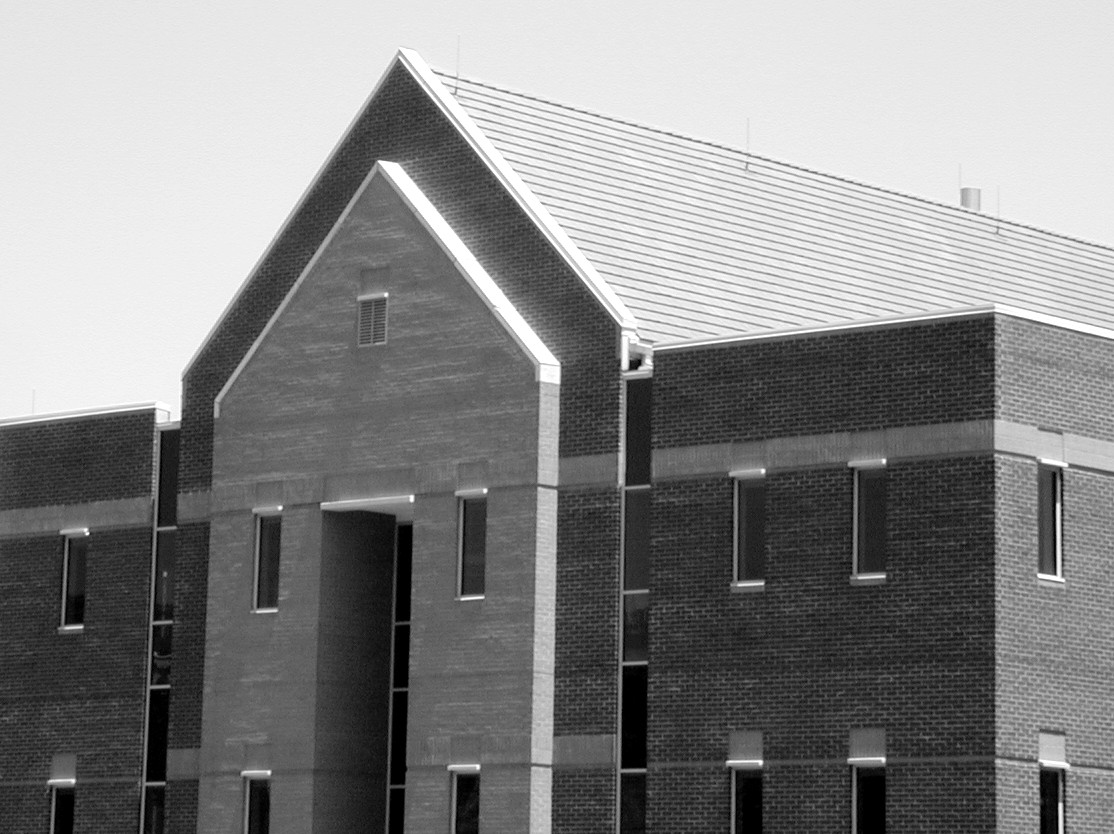
\includegraphics[width=\linewidth]{./images/9/building.jpg}}
            \caption{\small{Original image}}\label{diagram:building}
        \end{minipage}
    \end{figure}


    \begin{figure}[!htb]\centering
        \begin{minipage}{0.8\textwidth}
            \frame{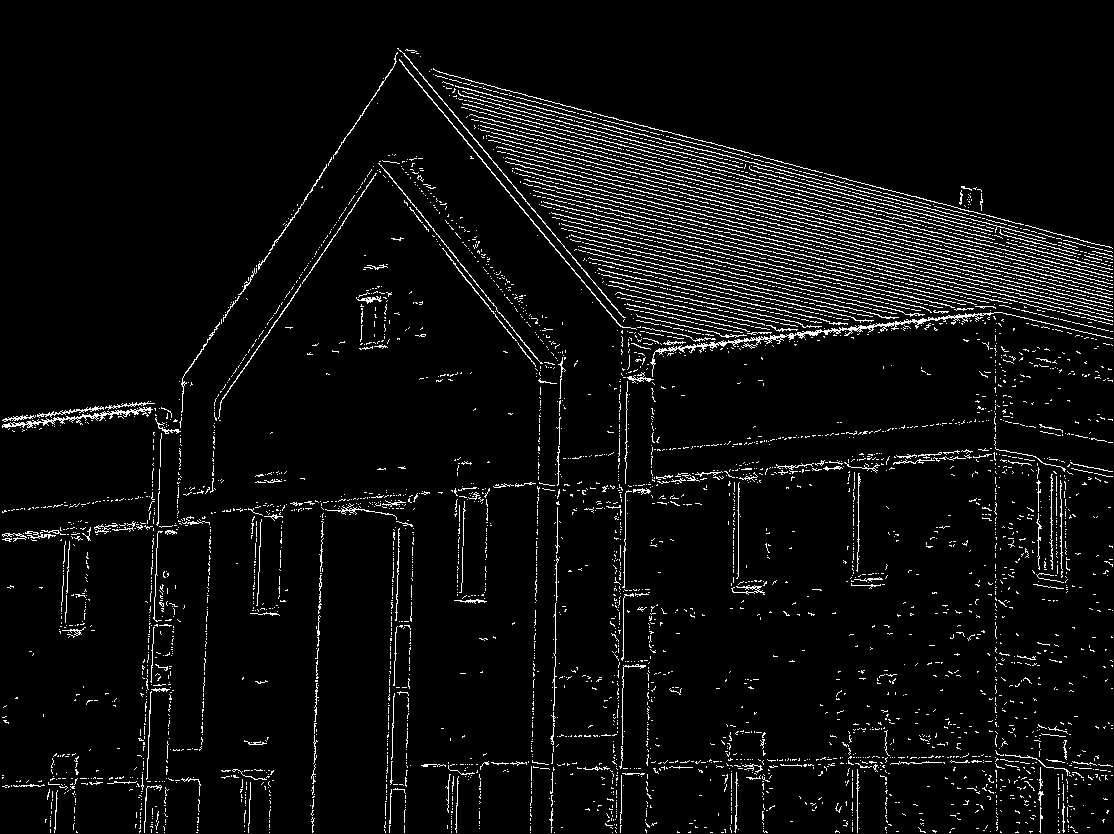
\includegraphics[width=\linewidth]{./images/9/roberts.jpg}}
            \caption{\small{Roberts}}\label{diagram:roberts}
        \end{minipage}
    \end{figure}

\subsection{Prewitt}

    \textbf{python canny.py --prewitt -s 4 --tl 0.04 --th 0.10 building.tif}

    \begin{figure}[!htb]\centering
        \begin{minipage}{0.8\textwidth}
            \frame{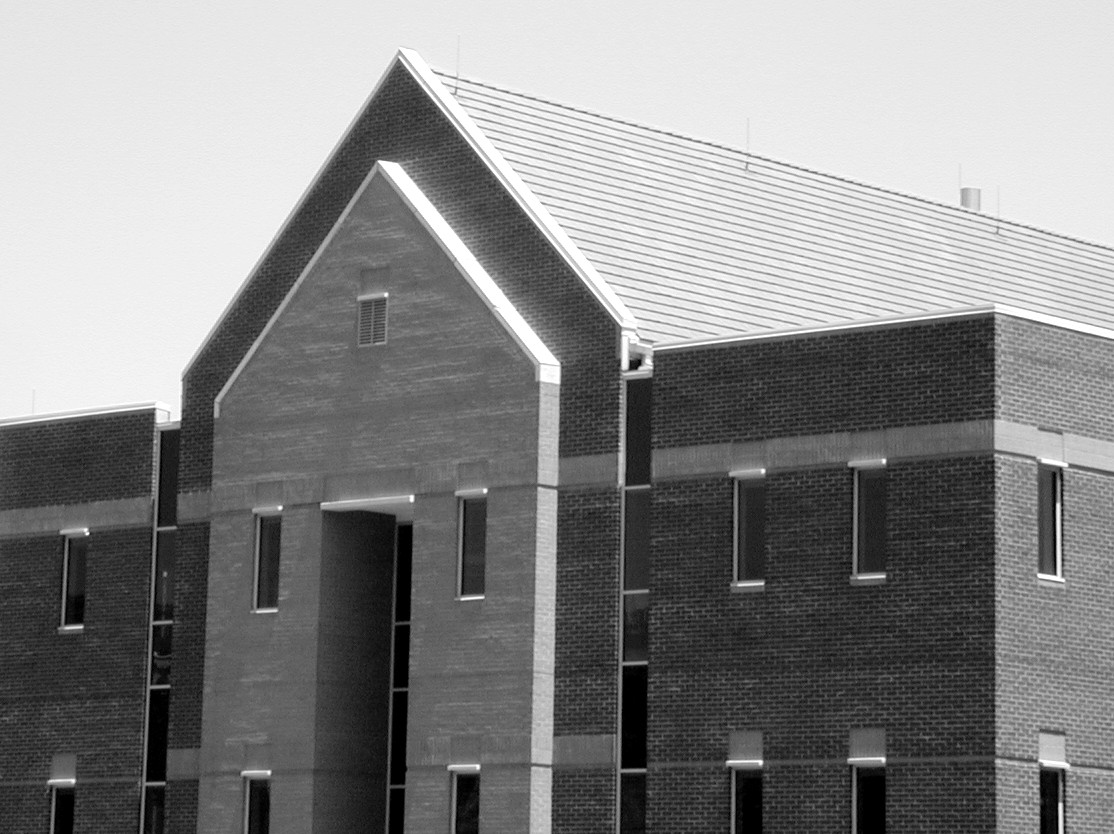
\includegraphics[width=\linewidth]{./images/9/building.jpg}}
            \caption{\small{Original image}}\label{diagram:building}
        \end{minipage}
    \end{figure}

    \begin{figure}[!htb]\centering
        \begin{minipage}{0.8\textwidth}
            \frame{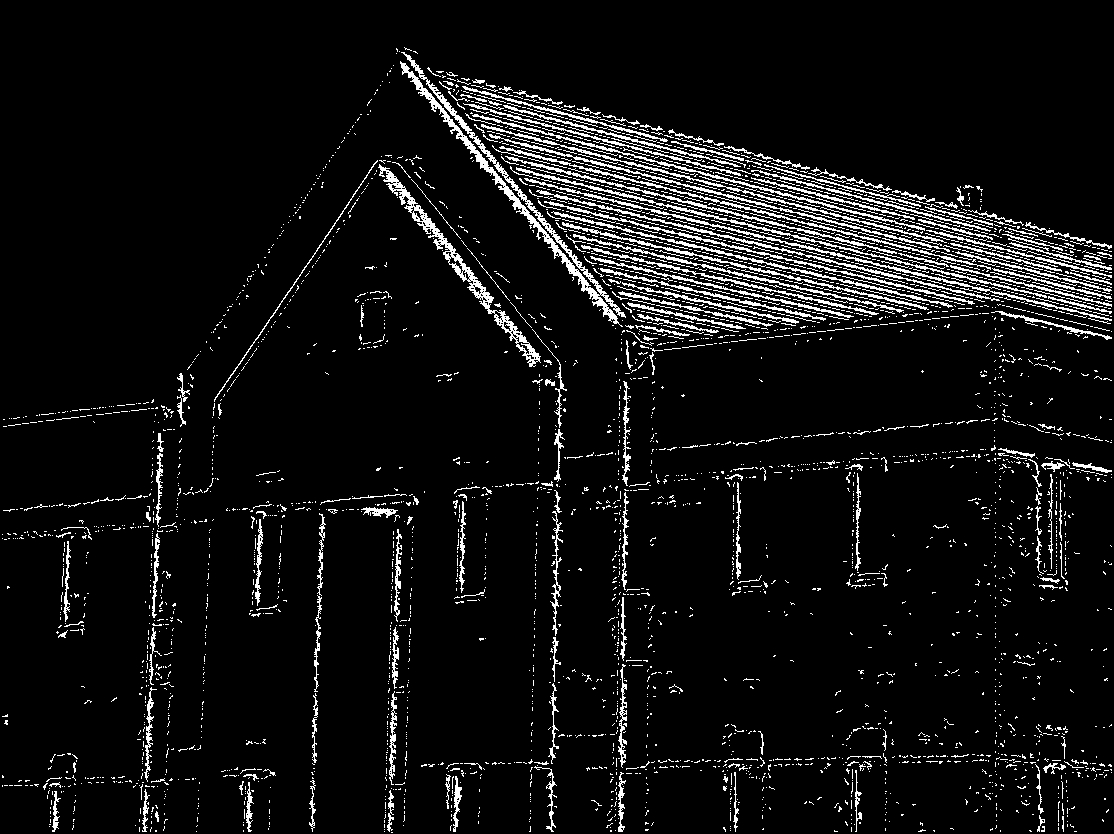
\includegraphics[width=\linewidth]{./images/9/prewitt.jpg}}
            \caption{\small{Prewitt}}\label{diagram:prewitt}
        \end{minipage}
    \end{figure}

\subsection{Sobel}

    \textbf{python canny.py --sobel -s 4 --tl 0.04 --th 0.10 building.tif}

    \begin{figure}[!htb]\centering
        \begin{minipage}{0.8\textwidth}
            \frame{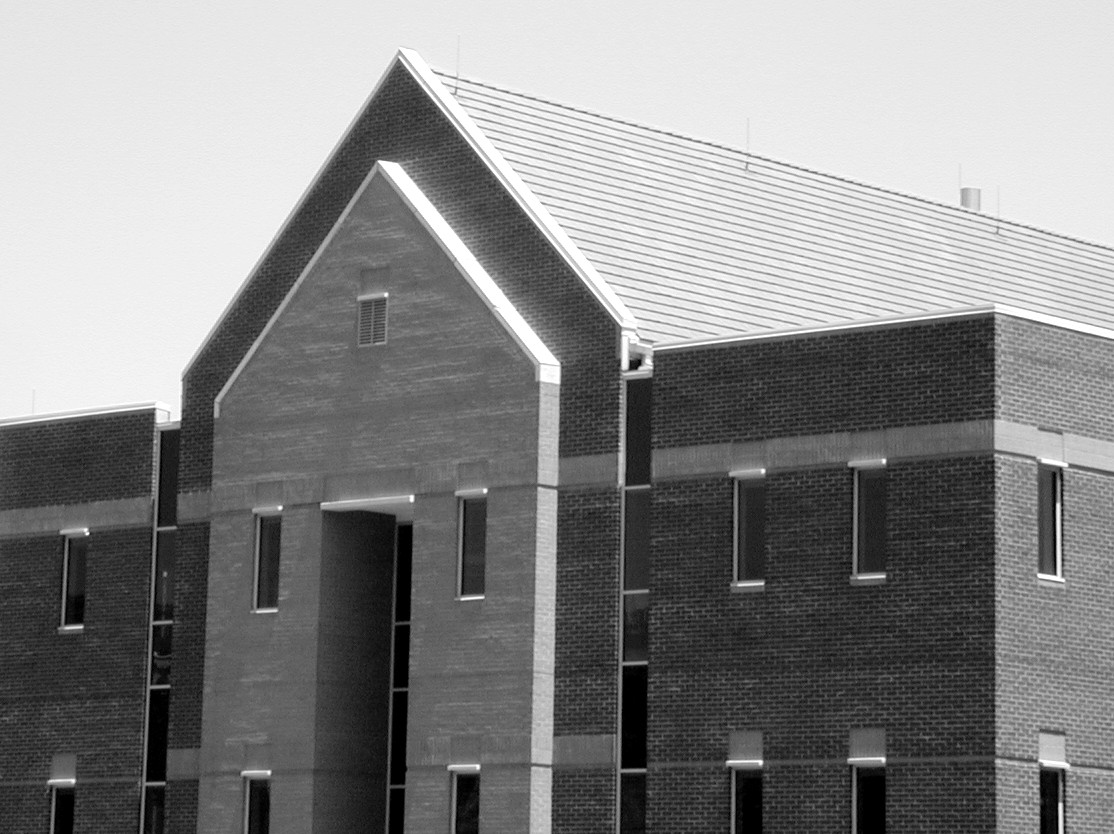
\includegraphics[width=\linewidth]{./images/9/building.jpg}}
            \caption{\small{Original image}}\label{diagram:building}
        \end{minipage}
    \end{figure}

    \begin{figure}[!htb]\centering
        \begin{minipage}{0.8\textwidth}
            \frame{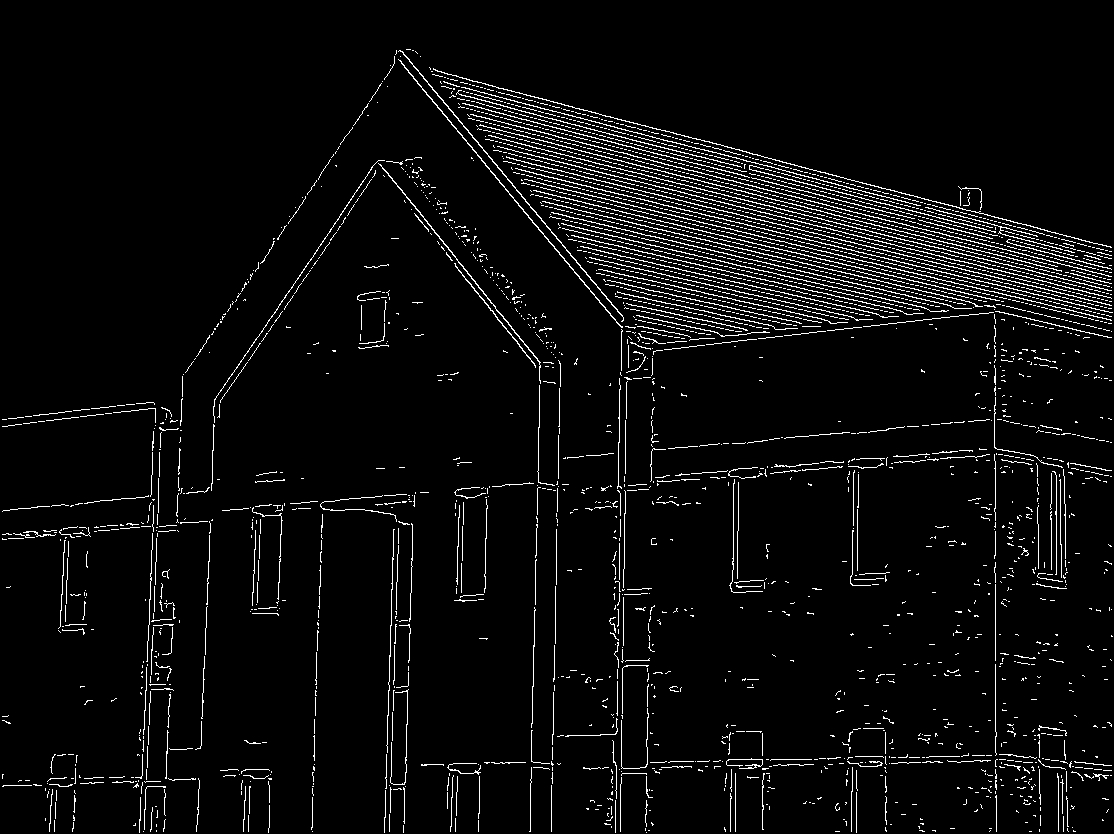
\includegraphics[width=\linewidth]{./images/9/sobel.jpg}}
            \caption{\small{Sobel}}\label{diagram:sobel}
        \end{minipage}
    \end{figure}


\section{Thresholding segmentation}

    \begin{figure}[!htb]\centering
        \begin{minipage}{0.6\textwidth}
            \frame{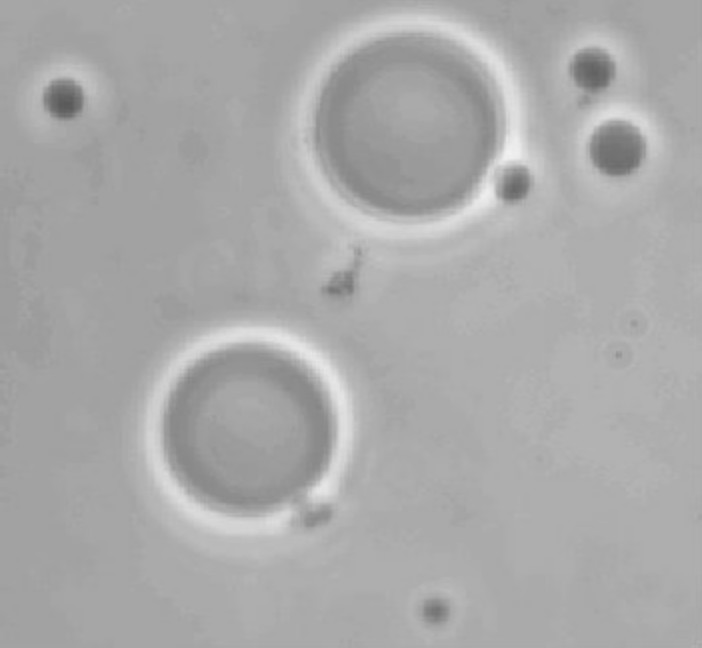
\includegraphics[width=\linewidth]{./images/9/polymersomes.jpg}}
            \caption{\small{Original image}}\label{diagram:polymersomes}
        \end{minipage}
    \end{figure}

\pagebreak

\subsection{Otsu}

    \begin{figure}[!htb]\centering
        \begin{minipage}{0.6\textwidth}
            \frame{
\includegraphics[width=\linewidth]{./images/9/otsu.jpg}}
            \caption{\small{Otsu}}\label{diagram:otsu}
        \end{minipage}
    \end{figure}

\subsection{Global thresholding}

    \begin{figure}[!htb]\centering
        \begin{minipage}{0.6\textwidth}
            \frame{
\includegraphics[width=\linewidth]{./images/9/gthresholding.jpg}}
            \caption{\small{Global thresholding}}\label{diagram:gthresholding}
        \end{minipage}
    \end{figure}


